\chapter{Specific Requirements}
This section is devoted to a specific description of every kind of requirement the
system has to deal with in order to achieve all the functionalities described.
\section{External interface Requirements}
\subsection{User Interfaces}
The mobile app is the interface which permit customers to enjoy CLup services. Whether installed on a smartphone or on a ticketing kiosk, it is the only way
for a customer to use CLup.
User interface mockups of most important pages of the app are shown below.

\vspace{0.5cm}
\begin{minipage}{.5\textwidth}
	\centering
	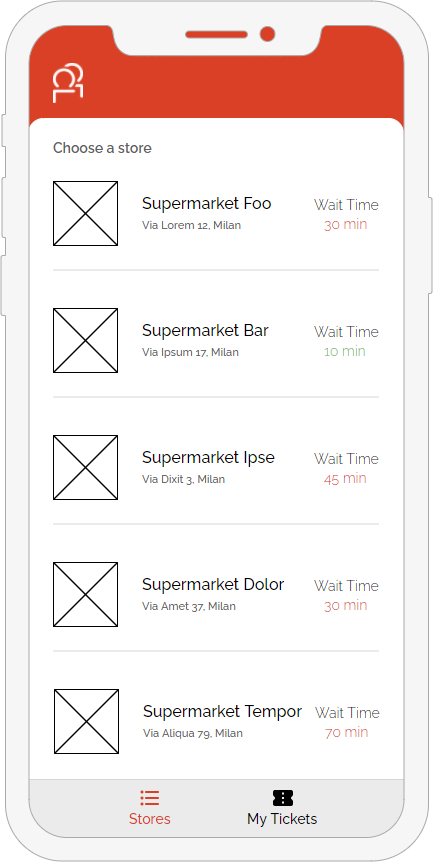
\includegraphics[scale=0.8]{home}
	\captionsetup{type=figure}
	\caption{App home.}
\end{minipage}%
\begin{minipage}{.5\textwidth}
	\centering
	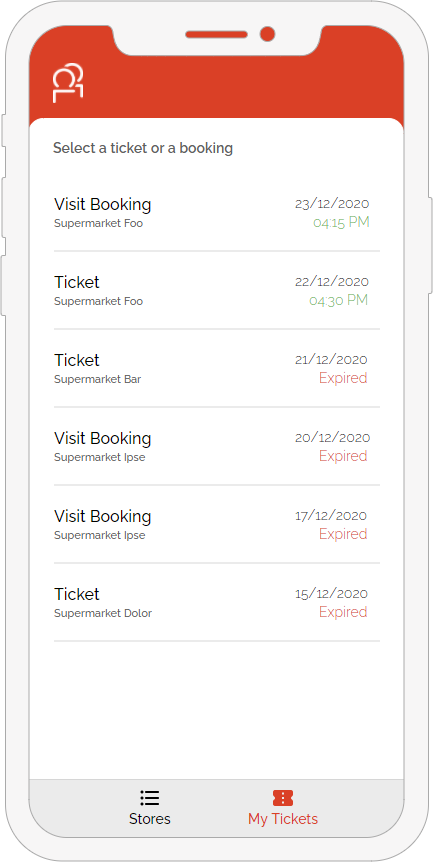
\includegraphics[scale=0.8]{my_tickets}
	\captionsetup{type=figure}
	\caption{Tickets list.}
\end{minipage}

\clearpage

\begin{minipage}{.5\textwidth}
	\centering
	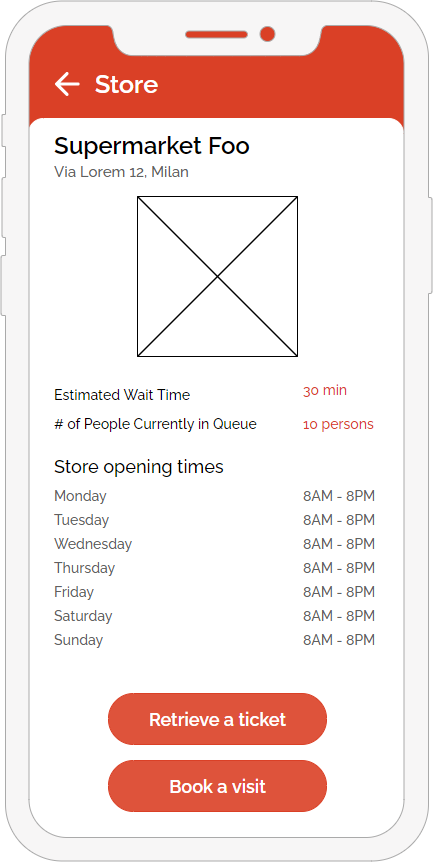
\includegraphics[scale=0.8]{store}
	\captionsetup{type=figure}
	\caption{Store page.}
\end{minipage}%
\begin{minipage}{.5\textwidth}
	\centering
	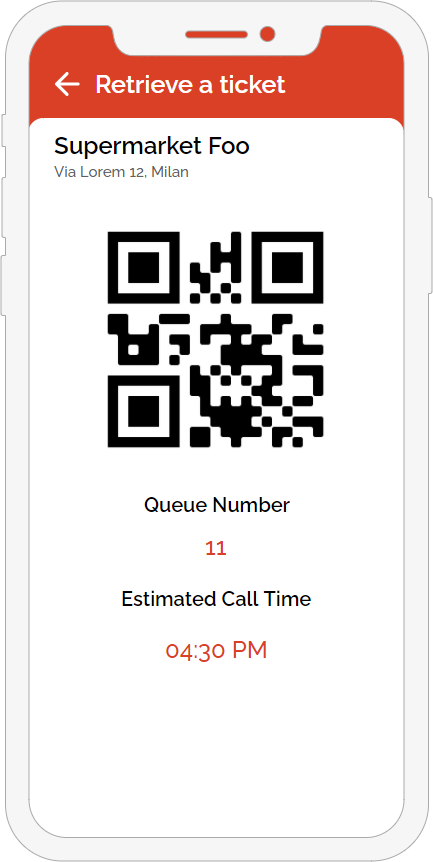
\includegraphics[scale=0.8]{ticket}
	\captionsetup{type=figure}
	\caption{Ticket Retrieved.}
\end{minipage}

\vspace{1cm}

\begin{minipage}{.5\textwidth}
	\centering
	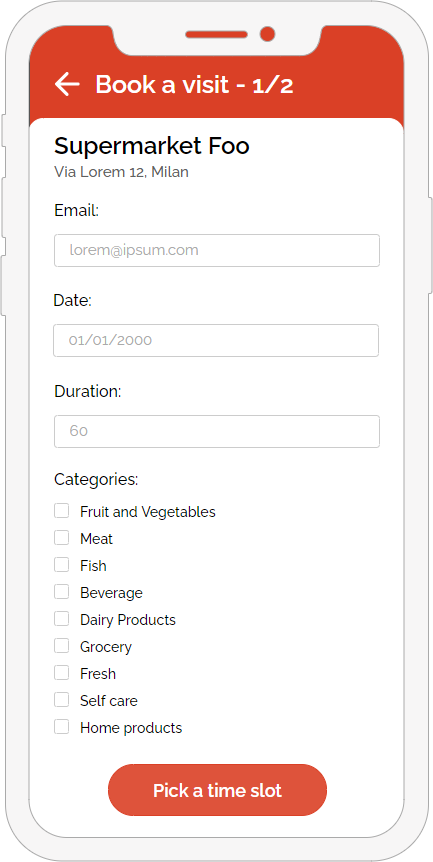
\includegraphics[scale=0.8]{book1}
	\captionsetup{type=figure}
	\caption{Book a visit (1/2).}
\end{minipage}%
\begin{minipage}{.5\textwidth}
	\centering
	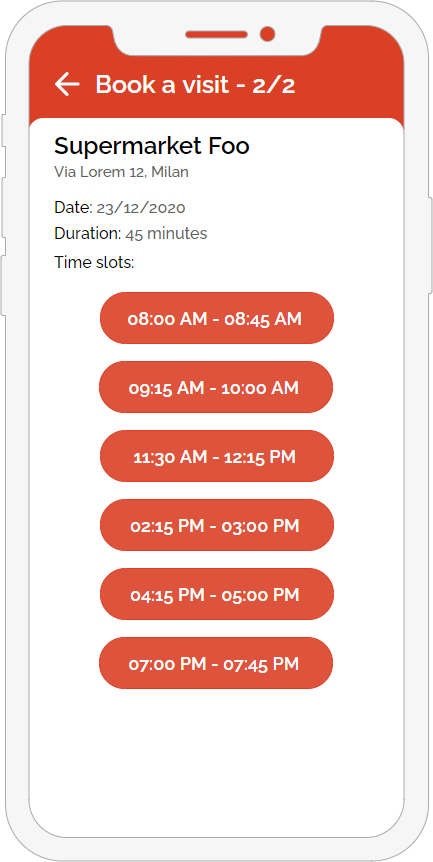
\includegraphics[scale=0.8]{book2}
	\captionsetup{type=figure}
	\caption{Book a visit (2/2).}
\end{minipage}

\vspace{1cm}

\begin{figure}[H]
	\centering
	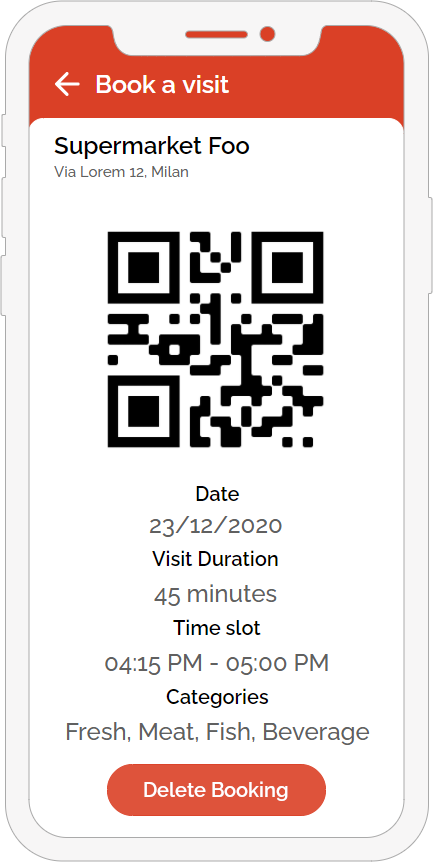
\includegraphics[scale=0.8]{book3}
	\caption{Visit booked.}
\end{figure}

\clearpage

Store managers and store employees use a web based interface for enjoying CLup features. The CLup admins can login at the same interface as well.
User interface mockups of most important pages of the web dashboard are shown below.
\vspace{0.5cm}
\begin{figure}[H]
	\centering
	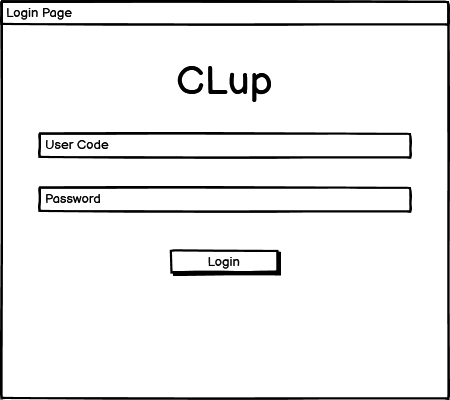
\includegraphics[width=0.64\linewidth]{login}
	\caption{Dashboard login.}
\end{figure}
\begin{figure}[H]
	\centering
	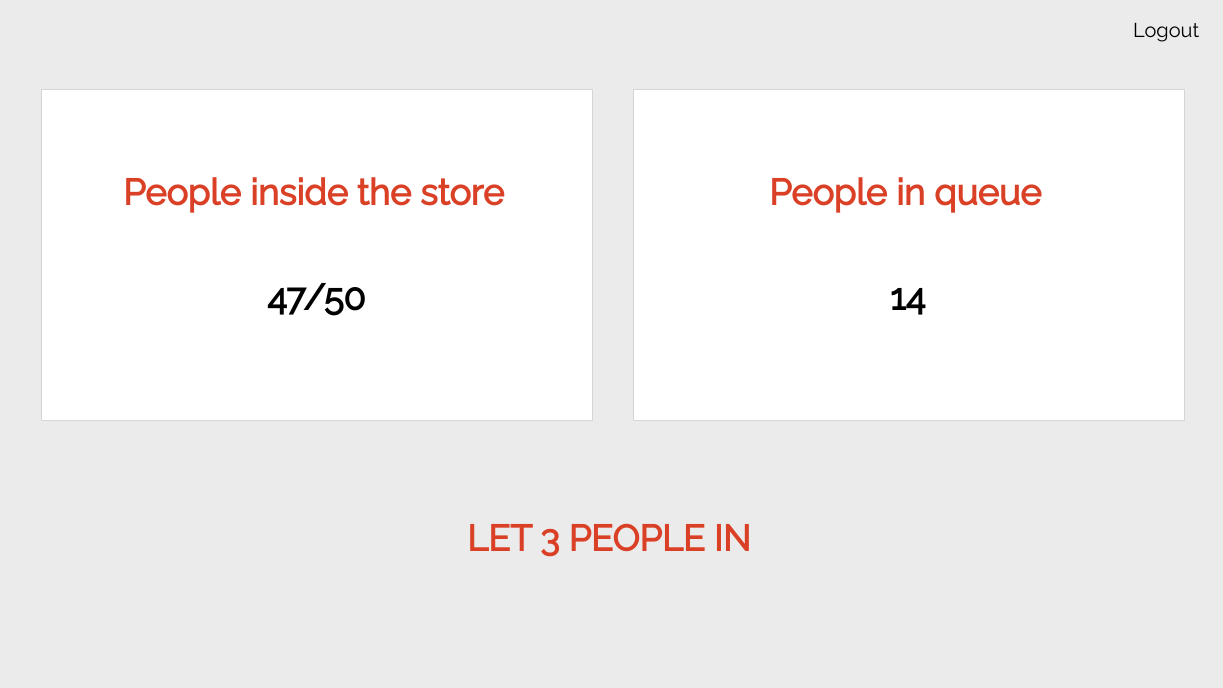
\includegraphics[width=0.64\linewidth]{employee}
	\caption{Employee homepage.}
\end{figure}
\begin{figure}[H]
	\centering
	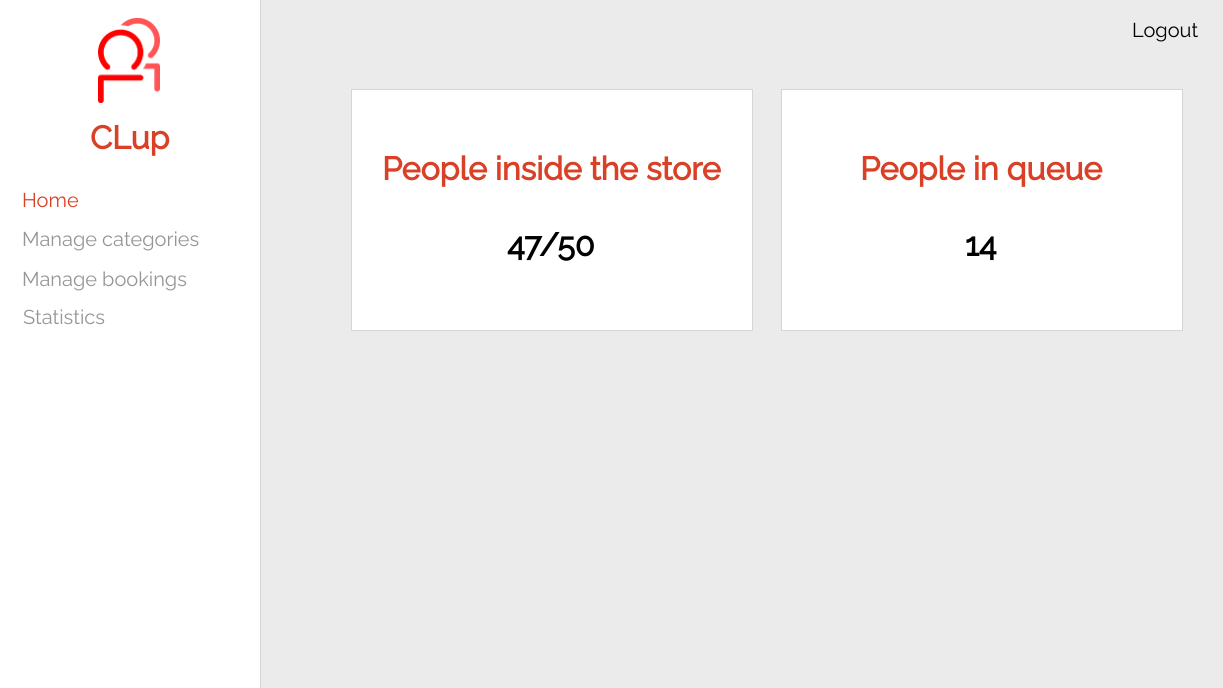
\includegraphics[width=0.64\linewidth]{dashboard1}
	\caption{Manager homepage.}
\end{figure}
\begin{figure}[H]
	\centering
	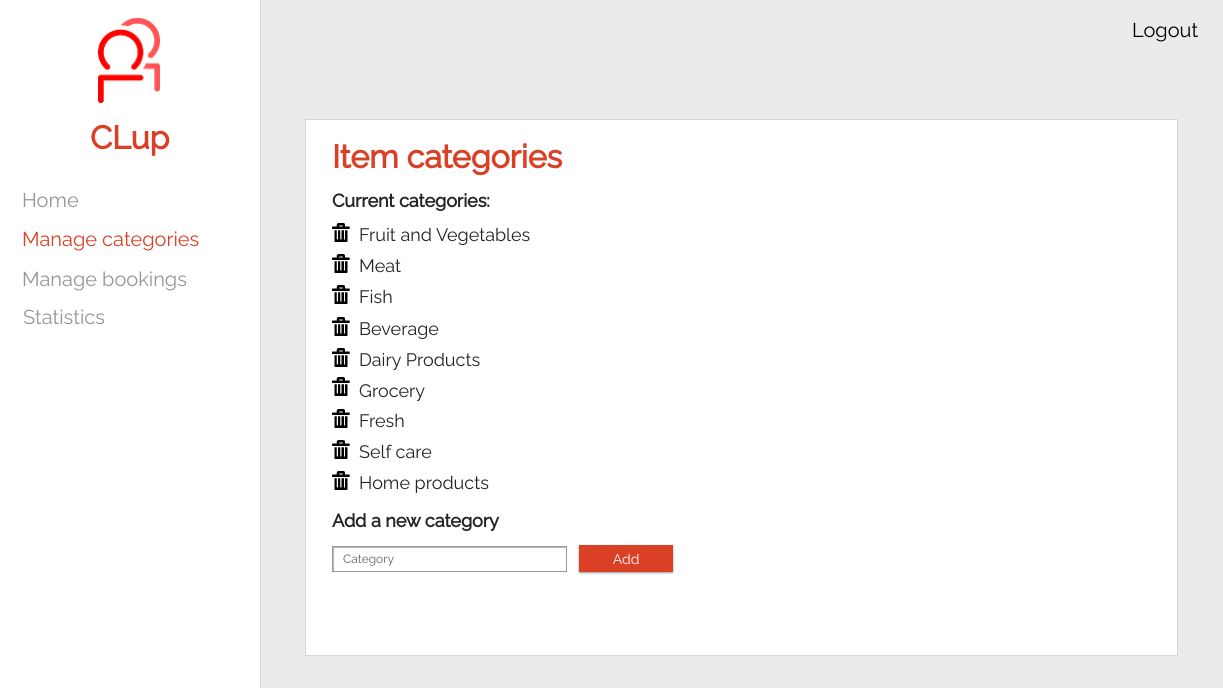
\includegraphics[width=0.64\linewidth]{dashboard2}
	\caption{Item categories page.}
\end{figure}
\begin{figure}[H]
	\centering
	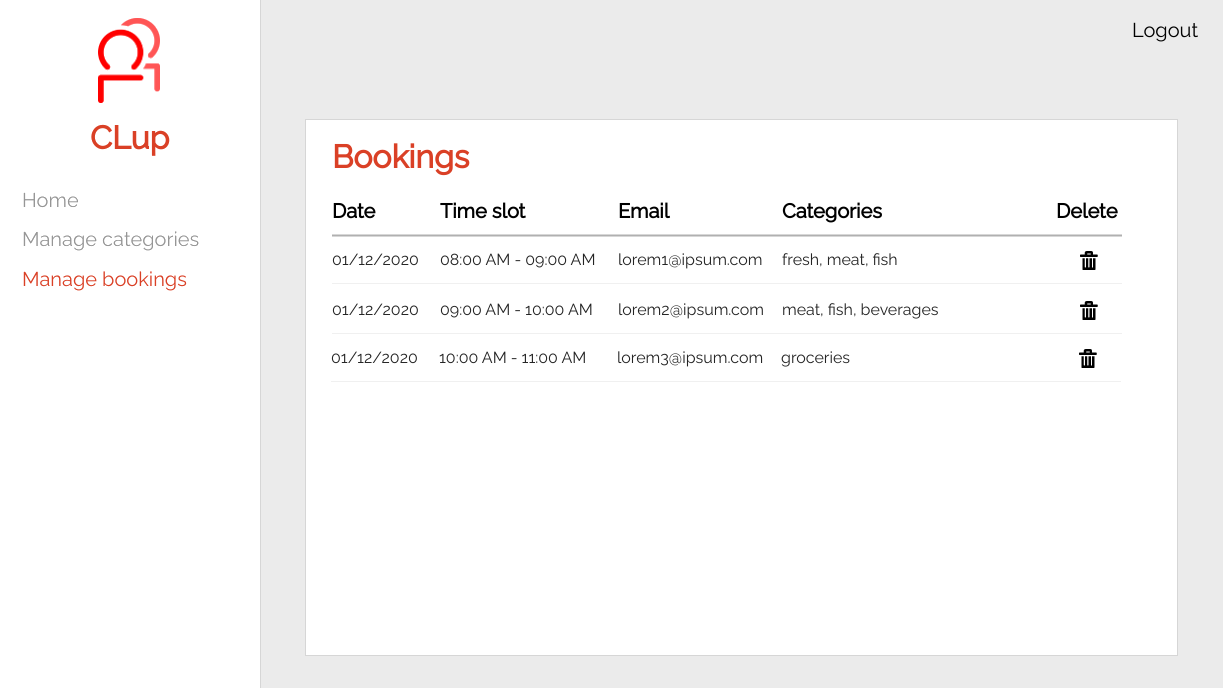
\includegraphics[width=0.64\linewidth]{dashboard3}
	\caption{Bookings list page.}
\end{figure}
\begin{figure}[H]
	\centering
	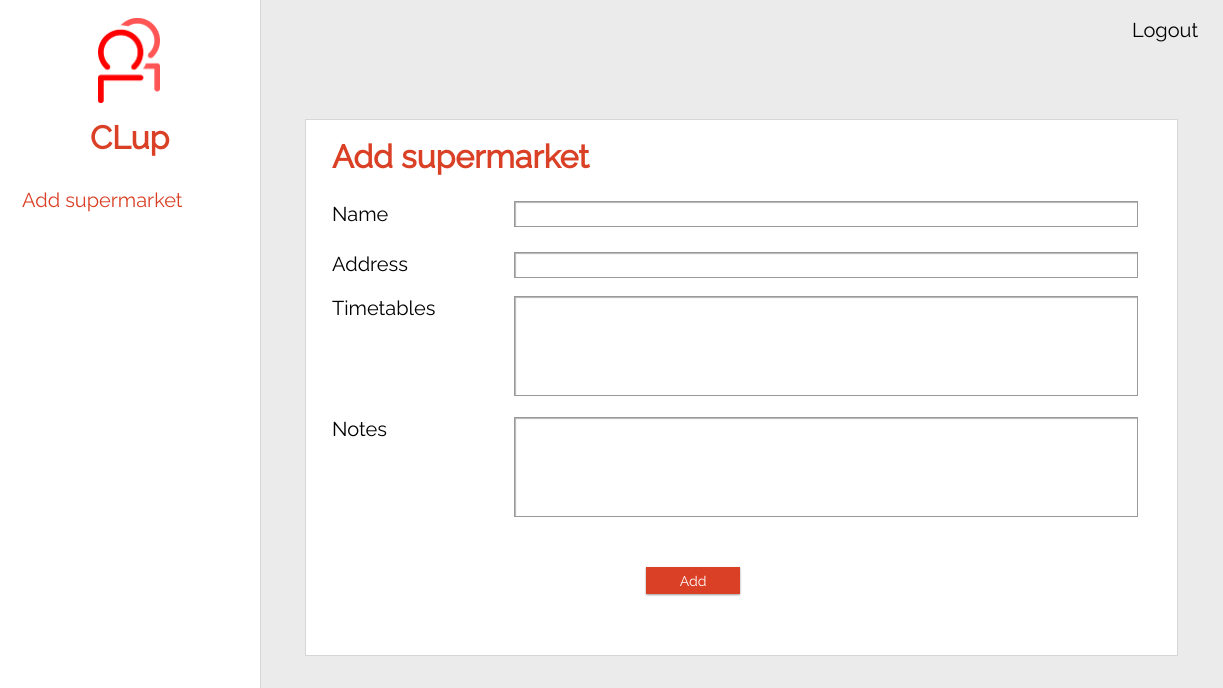
\includegraphics[width=0.64\linewidth]{new_store}
	\caption{Admin new supermarket page.}
\end{figure}

\clearpage

\subsection{Hardware Interfaces}
In addition to interfacing with computers (via a web browser), Clup interfaces with smartphones and their GPS module.
\subsection{Software Interfaces}
The system interfaces with a external map API for computing the distance between current place and store. It also permit to receive data
about QR codes via the public API.
\subsection{Communication Interfaces}
All the communications from and to CLup are made via HTTPS.

\section{Functional Requirements}
In this section, it is given a complete description of the functional requirements of the system.

    \subsection{Requirements}
    \subsubsection{Customer}
        \begin{enumerate}[series=requirements, label=\textbf{R.\arabic*}, leftmargin=+.3in]
            \item \itemtext{req:custQueue}{The system shall allow customers to line-up remotely in a store queue.}
            \item \itemtext{req:custTicket}{The system shall generate a new ticket when a customer enters a queue.}
            \item \itemtext{req:custTicketKiosk}{The system shall allow customers which do not have a smartphone to get a ticket in place.}
            \item \itemtext{req:custNum}{The system shall allow customers to view the number of people lined up in a queue.}
            \item \itemtext{req:custTime}{The system shall give customers an estimated waiting time.}
            \item \itemtext{req:custGps}{The system shall retrieve the GPS position while the user is subscribed to a queue.}
            \item \itemtext{req:custLeave}{The system shall allow customers to leave a queue.}
            \item \itemtext{req:custFilter}{The system shall allow customers to filter stores by name.}
            \item \itemtext{req:custTtl}{The system shall notify customers when it's time to leave for the store.}
            \item \itemtext{req:custBook}{The system shall allow customers to book-a-visit to the store and send them the receipt via email.}
            \item \itemtext{req:custItems}{The system shall allow book-a-visit customers to specify the main categories of item they intend to buy.}
            \item \itemtext{req:custDelete}{The system shall allow customers to delete a booked visit.}
            \item \itemtext{req:custNotifyDelete}{The system shall notify customers when a ticket or booked visit is deleted.}
        \end{enumerate}

    \subsubsection{Store manager}
    \begin{enumerate}[resume*=requirements]
        \item \itemtext{req:mngLogin}{A registered store manager must be able to login to the system by using his/her credentials.}
        \item \itemtext{req:mngViewStore}{The system shall allow store managers to view the current status of people inside the store.}
        \item \itemtext{req:mngViewQueue}{The system shall allow store managers to view the current status of people in the queue.}
         \item \itemtext{req:mngViewBook}{The system shall allow store managers to view the booked visits to the store.}
        \item \itemtext{req:mngCapStore}{The system shall allow store managers to set a maximum cap of people inside the store.}
        \item \itemtext{req:mngDeleteTickets}{The system shall allow store managers to delete tickets and booked visits.}
    \end{enumerate}

    \subsubsection{Store staff}
    \begin{enumerate}[resume*=requirements]
        \item \itemtext{req:stfLogin}{A registered store staff must be able to login to the system by using his/her credentials.}
        \item \itemtext{req:stfViewStore}{The system shall allow store staff to view the current status of people inside the store.}
        \item \itemtext{req:stfViewQueue}{The system shall allow store staff to view the current status of people in the queue.}
    \end{enumerate}

    \subsubsection{CLup admin}
    \begin{enumerate}[resume*=requirements]
        \item \itemtext{req:admRegister}{The system shall allow CLup admins to register new supermarkets.}
        \item \itemtext{req:admCredentials}{The system shall generate new manager and staff credential for each supermarket registered.}
    \end{enumerate}

    \subsection{Goal mapping on requirements}

    \begin{description}


        \item \printitem{goal:avoidQueue}

        \begin{description}

        	\item \printitem{goal:custHazardSit}

			\printitem{req:custQueue}
			\printitem{req:custNum}
			\printitem{req:custTime}
			\printitem{req:custTtl}
			\printitem{req:custBook}
			\printitem{req:custItems}

			\printitem{dom:smartphone}
			\printitem{dom:categories}
			\printitem{dom:custEmail}
			\printitem{dom:oneToOneQr}
			\printitem{dom:timeArrival}


			\item \printitem{goal:storeHazardSit}

			\printitem{req:mngViewStore}
			\printitem{req:mngViewQueue}
			\printitem{req:mngViewBook}
			\printitem{req:mngCapStore}
			\printitem{req:mngDeleteTickets}
			\printitem{req:stfViewStore}
			\printitem{req:stfViewQueue}

			\printitem{dom:categories}
			\printitem{dom:oneToOneQr}
			\printitem{dom:internetStores}
			\printitem{dom:employeeEntrance}
			\printitem{dom:timeArrival}
			\printitem{dom:capStores}


            \item \printitem{goal:shortenTime}

           	\printitem{req:custQueue}
           	\printitem{req:custNum}
           	\printitem{req:custTime}
           	\printitem{req:custTtl}
           	\printitem{req:custBook}

           	\printitem{dom:smartphone}
           	\printitem{dom:workingGps}
           	\printitem{dom:gpsPrecision}
           	\printitem{dom:bringSmartphone}
           	\printitem{dom:employeeEntrance}
           	\printitem{dom:qrServiceReliable}
           	\printitem{dom:qrServiceApi}
           	\printitem{dom:timeArrival}


            \item \printitem{goal:arriveOnTime}

           	\printitem{req:custQueue}
           	\printitem{req:custNum}
           	\printitem{req:custTime}
           	\printitem{req:custGps}
           	\printitem{req:custTtl}
           	\printitem{req:custBook}

           	\printitem{dom:smartphone}
           	\printitem{dom:workingGps}
           	\printitem{dom:gpsPrecision}
           	\printitem{dom:bringSmartphone}
           	\printitem{dom:timeArrival}
		\end{description}

        \item \printitem{goal:otherTasks}

       	\printitem{req:custQueue}
       	\printitem{req:custNum}
       	\printitem{req:custTime}
       	\printitem{req:custTtl}
       	\printitem{req:custBook}

       	\printitem{dom:smartphone}
       	\printitem{dom:workingGps}
       	\printitem{dom:gpsPrecision}
       	\printitem{dom:custEmail}
       	\printitem{dom:bringSmartphone}
       	\printitem{dom:timeArrival}


        \item \printitem{goal:easyExp}

       	\printitem{req:custTicket}
       	\printitem{req:custNum}
       	\printitem{req:custTime}
       	\printitem{req:custLeave}
       	\printitem{req:custFilter}
       	\printitem{req:custBook}
       	\printitem{req:custDelete}
       	\printitem{req:custNotifyDelete}

       	\printitem{dom:smartphone}
       	\printitem{dom:workingGps}
       	\printitem{dom:uniqueName}
       	\printitem{dom:qrServiceReliable}
       	\printitem{dom:storeRegistered}
       	\printitem{dom:storeKiosk}


        \item \printitem{goal:enjoyService}

       	\printitem{req:custQueue}
       	\printitem{req:custTicketKiosk}
       	\printitem{req:custBook}

       	\printitem{dom:smartphone}
       	\printitem{dom:internetStores}
       	\printitem{dom:storeRegistered}
       	\printitem{dom:storeKiosk}


        \item \printitem{goal:monitorAccess}

       	\printitem{req:mngLogin}
       	\printitem{req:mngViewStore}
       	\printitem{req:mngViewQueue}
       	\printitem{req:mngViewBook}
       	\printitem{req:stfLogin}
       	\printitem{req:stfViewStore}
       	\printitem{req:stfViewQueue}
       	\printitem{req:admRegister}
       	\printitem{req:admCredentials}

       	\printitem{dom:internetStores}
       	\printitem{dom:employeeEntrance}
       	\printitem{dom:storeRegistered}
       	\printitem{dom:capStores}


        \item \printitem{goal:knowInAdvance}

       	\printitem{req:mngViewStore}
       	\printitem{req:mngViewQueue}
       	\printitem{req:mngViewBook}
       	\printitem{req:stfViewStore}
       	\printitem{req:stfViewQueue}

       	\printitem{dom:smartphone}
       	\printitem{dom:categories}
       	\printitem{dom:internetStores}
       	\printitem{dom:storeRegistered}


        \item \printitem{goal:limitNumber}

       	\printitem{req:mngCapStore}
       	\printitem{req:mngDeleteTickets}

       	\printitem{dom:smartphone}
       	\printitem{dom:categories}
       	\printitem{dom:internetStores}
       	\printitem{dom:storeRegistered}
       	\printitem{dom:timeArrival}
       	\printitem{dom:capStores}

    \end{description}

    \subsection{Scenarios}

    \subsection{Use cases description}
    Use cases capture functional requirements of a system from the users' perspective.

	\begin{table}[H]
    	\centering
		\begin{tabular}{@{}p{0.25\linewidth}p{0.71\linewidth}@{}}
			\toprule
			\textbf{Name} & Retrieve ticket \\

			\midrule
			\textbf{ID} & \usecaseindex ~\\
			\midrule
			\textbf{Actors} & Customer \\
			\midrule
			\textbf{Entry conditions} &
				\begin{itemize}[leftmargin=.4cm,noitemsep,topsep=0pt,before=\vspace{-3mm},after=\vspace{-4mm}]
					\item The customer has installed the application on their device;
					\item The application is running.
				\end{itemize} \\
			\midrule
			\textbf{Flow of events} &
				\begin{enumerate}[label=\roman*.,leftmargin=.5cm,noitemsep,topsep=0pt,before=\vspace{-3mm},after=\vspace{-4mm}]
					\item The customer selects a store from the home page;
					\item The customer presses the "Retrieve Ticket" button.
				\end{enumerate} \\
			\midrule
			\textbf{Exit conditions} & The customer has retrieved a ticket for the selected store. \\
			\midrule
			\textbf{Exceptions} & If the customer has already retrieved a ticket for a store, the system displays an error message telling the customer they cannot get more than one ticket simultaneously. \\

			\bottomrule
		\end{tabular}
		\caption{\textit{Retrieve ticket} use case description.}
	\end{table}

	\begin{figure}[H]
		\centering
		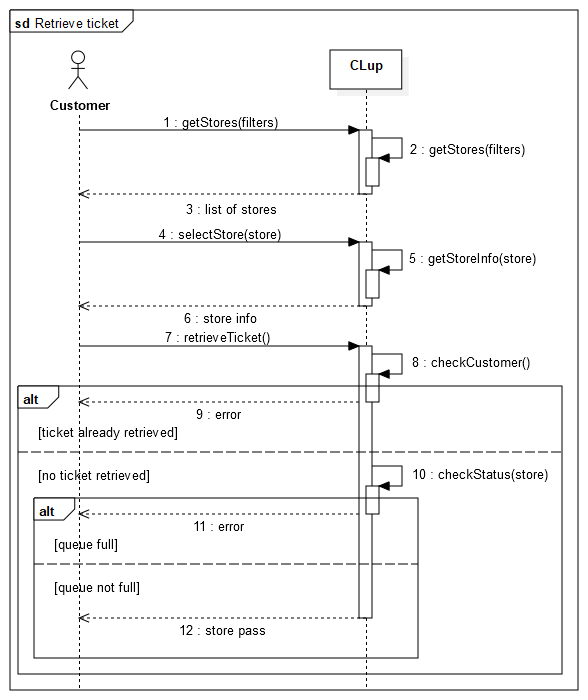
\includegraphics[width=\linewidth]{sd_retrieve_ticket}
		\caption{\textit{Retrieve ticket} sequence diagram.}
	\end{figure}

	\begin{table}[H]
    	\centering
    	\begin{tabular}{@{}p{0.25\linewidth}p{0.71\linewidth}@{}}
    		\toprule
    		\textbf{Name} & Book a visit \\

    		\midrule
    		\textbf{ID} & \usecaseindex ~\\
    		\midrule
    		\textbf{Actors} & Customer \\
    		\midrule
    		\textbf{Entry conditions} &
    		\begin{itemize}[leftmargin=.4cm,noitemsep,topsep=0pt,before=\vspace{-3mm},after=\vspace{-4mm}]
    			\item The customer has installed the application on their device;
    			\item The application is running.
    		\end{itemize} \\
    		\midrule
    		\textbf{Flow of events} &
    		\begin{enumerate}[label=\roman*.,leftmargin=.5cm,noitemsep,topsep=0pt,before=\vspace{-3mm},after=\vspace{-4mm}]
    			\item The customer selects a store from the home page;
    			\item The customer presses the "Book a visit" button;
    			\item The customer inserts their email address, the date, the approximate duration of the visit and the main categories of items they intend to buy;
    			\item The customer selects the time slot;
                \item The customer submits the form;
                \item The system shows to the customer the booked visit.
    		\end{enumerate} \\
    		\midrule
    		\textbf{Exit conditions} & The customer has retrieved a ticket for the selected store. \\
    		\midrule
    		\textbf{Exceptions} &
            \begin{itemize}[leftmargin=.4cm,noitemsep,topsep=0pt,before=\vspace{-3mm},after=\vspace{-4mm}]
                \item If the customer has already booked a visit to a store in a certain date, the system displays an error message telling the customer it cannot book again for the same day at the same store;
                \item If the customer selects a date so that there are no more available time slots, the system displays an error message telling the customer to select a different date.
            \end{itemize} \\

    		\bottomrule
    	\end{tabular}
    	\caption{\textit{Book a visit} use case description.}
    \end{table}

	\begin{figure}[H]
		\centering
		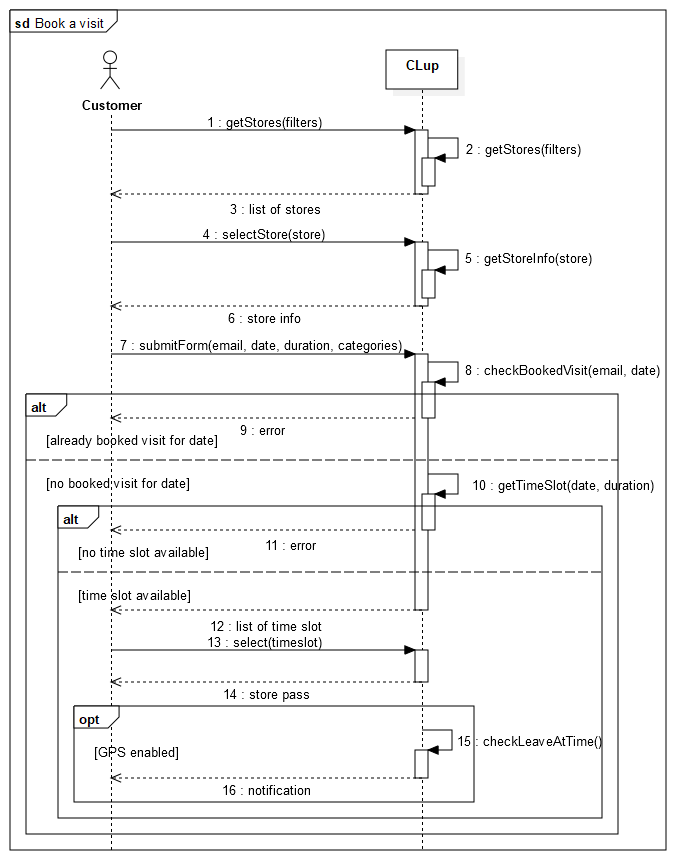
\includegraphics[width=\linewidth]{sd_book_a_visit}
		\caption{\textit{Book a visit} sequence diagram.}
	\end{figure}

	\begin{table}[H]
        \centering
        \begin{tabular}{@{}p{0.25\linewidth}p{0.71\linewidth}@{}}
            \toprule
            \textbf{Name} & Delete a store pass \\

            \midrule
            \textbf{ID} & \usecaseindex ~\\
            \midrule
            \textbf{Actors} & Customer \\
            \midrule
            \textbf{Entry conditions} &
            \begin{itemize}[leftmargin=.4cm,noitemsep,topsep=0pt,before=\vspace{-3mm},after=\vspace{-4mm}]
                \item The customer has installed the application on their device;
                \item The application is running.
            \end{itemize} \\
            \midrule
            \textbf{Flow of events} &
            \begin{enumerate}[label=\roman*.,leftmargin=.5cm,noitemsep,topsep=0pt,before=\vspace{-3mm},after=\vspace{-4mm}]
                \item The customer swipes to the "My Store Pass" page;
                \item The customer selects one of the available store passes;
                \item The customer presses the "Delete Store Pass" button;
                \item The customer selects "Yes" on the confirmation message;
                \item The customer is notified by the system that the store pass has been deleted successfully.
            \end{enumerate} \\
            \midrule
            \textbf{Exit conditions} & The customer has deleted successfully a store pass. \\
            \midrule
            \textbf{Exceptions} & If the customer has no store pass, the system displays a label: "No store pass available". \\
            \bottomrule
        \end{tabular}
        \caption{\textit{Delete a store pass} use case description.}
    \end{table}

	\begin{figure}[H]
		\centering
		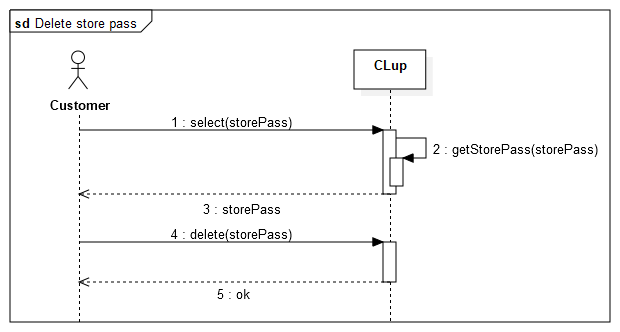
\includegraphics[width=\linewidth]{sd_delete_store_pass}
		\caption{\textit{Delete a store pass} sequence diagram.}
	\end{figure}


	\begin{table}[H]
        \centering
        \begin{tabular}{@{}p{0.25\linewidth}p{0.71\linewidth}@{}}
            \toprule
            \textbf{Name} & Web platform login \\

            \midrule
            \textbf{ID} & \usecaseindex ~\\
            \midrule
            \textbf{Actors} & Store manager, Store employee, CLup admin \\
            \midrule
            \textbf{Entry conditions} &
            \begin{itemize}[leftmargin=.4cm,noitemsep,topsep=0pt,before=\vspace{-3mm},after=\vspace{-4mm}]
                \item The web platform is running.
            \end{itemize} \\
            \midrule
            \textbf{Flow of events} &
            \begin{enumerate}[label=\roman*.,leftmargin=.5cm,noitemsep,topsep=0pt,before=\vspace{-3mm},after=\vspace{-4mm}]
                \item The actor goes to the login page;
                \item The actor inserts their username and password;
                \item The actor submits the form.
            \end{enumerate} \\
            \midrule
            \textbf{Exit conditions} & The actor has successfully logged into the web platform. \\
            \midrule
            \textbf{Exceptions} &
            \begin{itemize}[leftmargin=.4cm,noitemsep,topsep=0pt,before=\vspace{-3mm},after=\vspace{-4mm}]
                \item If the username is not recognized by the system, the credentials are not registered or the username is incorrect. The system notifies the actor and the procedure is aborted.
                \item If the inserted password is wrong, the system notifies the actor and the procedure is aborted.
            \end{itemize} \\

            \bottomrule
        \end{tabular}
        \caption{\textit{Web platform login} use case description.}
    \end{table}

	\begin{figure}[H]
		\centering
		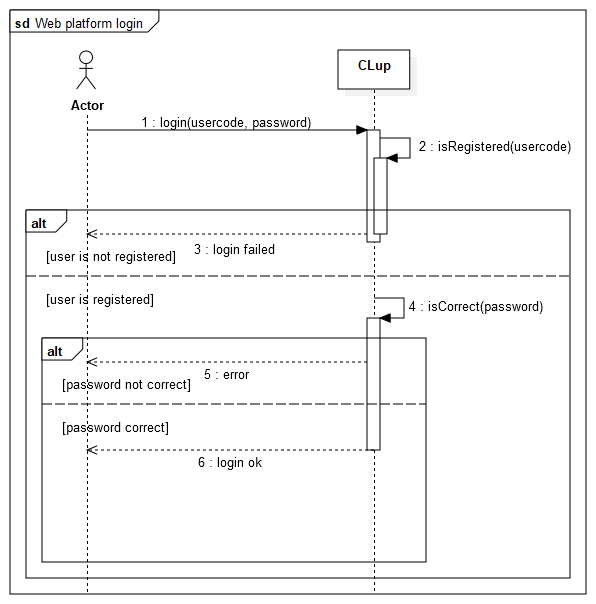
\includegraphics[width=\linewidth]{sd_web_platform_login}
		\caption{\textit{Web platform login} sequence diagram.}
	\end{figure}


	\begin{table}[H]
        \centering
        \begin{tabular}{@{}p{0.25\linewidth}p{0.71\linewidth}@{}}
            \toprule
            \textbf{Name} & Register new store \\

            \midrule
            \textbf{ID} & \usecaseindex ~\\
            \midrule
            \textbf{Actors} & CLup admin \\
            \midrule
            \textbf{Entry conditions} &
            \begin{itemize}[leftmargin=.4cm,noitemsep,topsep=0pt,before=\vspace{-3mm},after=\vspace{-4mm}]
                \item The web platform is running.
                \item The CLup admin is logged in.
                \item The CLup admin has been contacted by a store manager.
            \end{itemize} \\
            \midrule
            \textbf{Flow of events} &
            \begin{enumerate}[label=\roman*.,leftmargin=.5cm,noitemsep,topsep=0pt,before=\vspace{-3mm},after=\vspace{-4mm}]
                \item The CLup admin goes to the "Add supermarket" page;
                \item The CLup admin fills in the form providing store information: name, address, email and timetables.
                \item The CLup admin submits the form.
                \item The system generates credentials for the store managers and store employee and send them to the store via email.
            \end{enumerate} \\
            \midrule
            \textbf{Exit conditions} & The CLup admin has added a store to the platform. \\
            \midrule
            \textbf{Exceptions} &
            \begin{itemize}[leftmargin=.4cm,noitemsep,topsep=0pt,before=\vspace{-3mm},after=\vspace{-4mm}]
                \item If the store name is already used by another store, the system displays an error message asking the CLup admin to insert a different one.
            \end{itemize} \\

            \bottomrule
        \end{tabular}
        \caption{\textit{Register new store} use case description.}
    \end{table}

	\begin{figure}[H]
		\centering
		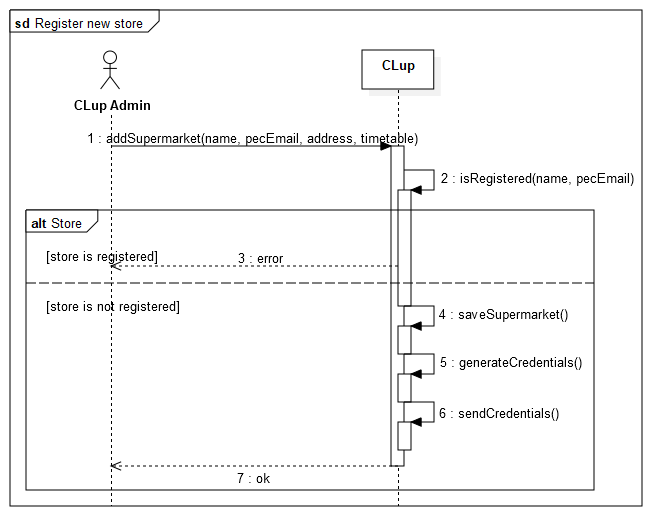
\includegraphics[width=\linewidth]{sd_register_new_store}
		\caption{\textit{Register new store} sequence diagram.}
	\end{figure}


	\begin{table}[H]
        \centering
        \begin{tabular}{@{}p{0.25\linewidth}p{0.71\linewidth}@{}}
            \toprule
            \textbf{Name} & Monitor bookings \\

            \midrule
            \textbf{ID} & \usecaseindex ~\\
            \midrule
            \textbf{Actors} & Store manager \\
            \midrule
            \textbf{Entry conditions} &
            \begin{itemize}[leftmargin=.4cm,noitemsep,topsep=0pt,before=\vspace{-3mm},after=\vspace{-4mm}]
                \item The web platform is running.
                \item The store manager is logged in.
            \end{itemize} \\
            \midrule
            \textbf{Flow of events} &
            \begin{enumerate}[label=\roman*.,leftmargin=.5cm,noitemsep,topsep=0pt,before=\vspace{-3mm},after=\vspace{-4mm}]
                \item The Store manager go to the "Manage bookings list" page;
                \item The Store manager can filter bookings by date, time slot and categories;
                \item The system provides to the store manager a list with all the bookings that match the filter. If no filter are provided, a full list of all the bookings is shown.
            \end{enumerate} \\
            \midrule
            \textbf{Exit conditions} & The Store manager view the bookings. \\
            \midrule
            \textbf{Exceptions} &
            \begin{itemize}[leftmargin=.4cm,noitemsep,topsep=0pt,before=\vspace{-3mm},after=\vspace{-4mm}]
                \item If no bookings are available, an error is prompted to the store manager.
            \end{itemize} \\

            \bottomrule
        \end{tabular}
        \caption{\textit{Monitor bookings} use case description.}
    \end{table}

	\begin{figure}[H]
		\centering
		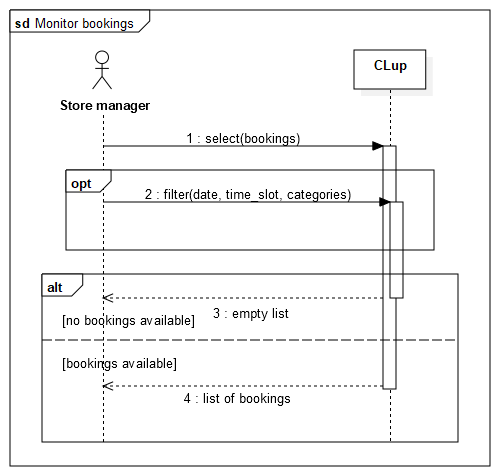
\includegraphics[width=\linewidth]{sd_monitor_bookings}
		\caption{\textit{Monitor bookings} sequence diagram.}
	\end{figure}


    \subsection{Traceability matrix}
    \begin{center}
        \begin{tabular}{@{}p{0.25\linewidth}cccc@{}}
            \toprule
            \textbf{Item} & \textbf{\ref{req:custQueue}} & \textbf{\ref{req:custTicket}}
            & \textbf{\ref{req:custTime}} & \textbf{\ref{req:custNum}}\\
            \midrule
            Lorem Ipsum & \cmark \\
            Dolor Sit & & & \cmark \\

            \bottomrule
        \end{tabular}
    \end{center}


\section{Performance Requirements}

\section{Design Constraints}

\section{Software System Attributes}